\documentclass[aspectratio=169,11pt]{beamer}
\usepackage[T1]{fontenc}
\usepackage{lmodern}
\usepackage{microtype}
\usepackage{amsmath,amssymb,mathtools}
\usepackage{booktabs,array}
\usepackage{tikz}
\usetikzlibrary{arrows.meta,positioning,calc}
\usepackage{hyperref}

\definecolor{navy}{HTML}{15324B}
\definecolor{teal}{HTML}{007C83}
\definecolor{gold}{HTML}{B57A00}
\definecolor{rose}{HTML}{9A3B47}
\definecolor{pale}{HTML}{F2F7F8}
\definecolor{ink}{HTML}{17212B}
\definecolor{muted}{HTML}{5B6770}

\usetheme{default}
\usecolortheme{default}
\setbeamercolor{normal text}{fg=ink,bg=white}
\setbeamercolor{structure}{fg=navy}
\setbeamercolor{frametitle}{fg=white,bg=navy}
\setbeamercolor{block title}{fg=white,bg=teal}
\setbeamercolor{block body}{fg=ink,bg=pale}
\setbeamercolor{block title alerted}{fg=white,bg=rose}
\setbeamercolor{block body alerted}{fg=ink,bg=rose!7}
\setbeamercolor{block title example}{fg=white,bg=gold!88!black}
\setbeamercolor{block body example}{fg=ink,bg=gold!8}
\setbeamerfont{title}{size=\fontsize{25}{29}\selectfont,series=\bfseries}
\setbeamerfont{subtitle}{size=\Large}
\setbeamerfont{frametitle}{size=\Large,series=\bfseries}
\setbeamerfont{block title}{size=\normalsize,series=\bfseries}
\setbeamerfont{footline}{size=\tiny}
\setbeamersize{text margin left=7mm,text margin right=7mm}
\setbeamertemplate{navigation symbols}{}
\setbeamertemplate{itemize item}{\color{teal}$\blacktriangleright$}
\setbeamertemplate{itemize subitem}{\color{gold}$\bullet$}
\setlength{\leftmargini}{5mm}
\setlength{\leftmarginii}{4mm}

\setbeamertemplate{frametitle}{
  \nointerlineskip
  \begin{beamercolorbox}[wd=\paperwidth,ht=9mm,dp=2.6mm,leftskip=7mm,rightskip=7mm]{frametitle}
    \insertframetitle
  \end{beamercolorbox}
}
\setbeamertemplate{footline}{
  \leavevmode
  \hbox{%
    \begin{beamercolorbox}[wd=.72\paperwidth,ht=3.2mm,dp=1.2mm,leftskip=7mm]{author in head/foot}
      \color{muted}Aouad, Lykouris, and Zhong (2026) --- Part II intuition lecture
    \end{beamercolorbox}%
    \begin{beamercolorbox}[wd=.28\paperwidth,ht=3.2mm,dp=1.2mm,rightskip=7mm plus1fil]{date in head/foot}
      \hfill\color{muted}\insertframenumber/\inserttotalframenumber
    \end{beamercolorbox}%
  }
}

\newcommand{\pos}[1]{\left(#1\right)_{+}}
\newcommand{\calP}{\mathcal{P}}
\newcommand{\calE}{\mathcal{E}}
\newcommand{\key}[1]{\textcolor{teal}{\textbf{#1}}}
\newcommand{\warning}[1]{\textcolor{rose}{\textbf{#1}}}
\newcommand{\econmeaning}[1]{%
  \begin{block}{Economic meaning}
  #1
  \end{block}}
\newcommand{\bottomline}[1]{%
  \begin{alertblock}{Bottom line}
  #1
  \end{alertblock}}

\title{Part II: Endogenous Skill}
\subtitle{Reading the equations as economic stories}
\author{Alexander Quispe\\[-1mm]\small\href{mailto:aquisper@caltech.edu}{aquisper@caltech.edu}}
\date{\small Human--AI Productivity Paradoxes}

\begin{document}

% ============================================================
% OPENING
% ============================================================

\begin{frame}[plain]
  \begin{tikzpicture}[remember picture,overlay]
    \fill[navy] (current page.south west) rectangle (current page.north east);
    \fill[gold] (current page.south west) rectangle ([xshift=18mm]current page.north west);
    \draw[teal,line width=1.5pt] ([xshift=24mm,yshift=-18mm]current page.north west)
      -- ([xshift=-16mm,yshift=-18mm]current page.north east);
  \end{tikzpicture}
  \vspace{15mm}
  {\usebeamerfont{title}\color{white}\inserttitle\par}
  \vspace{3mm}
  {\usebeamerfont{subtitle}\color{white!88}\insertsubtitle\par}
  \vspace{11mm}
  {\color{white}\large An intuition-first lecture on Section 4 of the tutorial\par}
  \vfill
  {\color{white}\insertauthor\par}
  \vspace{2mm}
  {\color{white!70}\insertdate\par}
\end{frame}

\begin{frame}{The paradox comes from the weights, not the groups}
At every fixed skill state, AI weakly raises optimized productivity:
\[
\frac{\partial p^\star(s_k,a)}{\partial a}\ge 0.
\]
Yet long-run productivity is a weighted average,
\[
\calP(a)=\sum_{k=1}^{N}\pi_k(a)p^\star(s_k,a),
\]
and the weights $\pi_k(a)$ also change with AI.
\bottomline{AI can improve productivity within every skill state while shifting enough probability toward low skill to reduce the aggregate.}
\end{frame}

\begin{frame}{Three questions organize the entire lecture}
\begin{enumerate}
  \item Why does more AI reduce the incentive to learn?
  \item How does lower effort become a worse long-run skill distribution?
  \item When can that composition loss dominate AI's direct productivity gain?
\end{enumerate}
\vspace{5mm}
\begin{exampleblock}{The answer in one line}
\centering
\large substitution $\longrightarrow$ deskilling $\longrightarrow$ composition reversal
\end{exampleblock}
\end{frame}

\begin{frame}{Recall the static result: AI first replaces effort}
At skill $s_k$, optimal effort is
\[
\boxed{e_k(a)=e^\star(s_k,a)=\pos{x^\star-s_k-a}.}
\]
As long as effort is positive,
\[
\frac{d e_k(a)}{da}=-1.
\]
\econmeaning{One additional unit of AI replaces exactly one unit of human effort until effort reaches zero. Total productive input remains at $x^\star$ during this replacement phase.}
\end{frame}

\begin{frame}{At a fixed skill, AI never lowers output}
The optimized state-level productivity is
\[
\boxed{p_k^\star(a)=\max\{p(x^\star),\,p(s_k+a)\}.}
\]
Therefore,
\[
\frac{d p_k^\star(a)}{da}\ge 0.
\]
\econmeaning{The paradox cannot be a failure of the static optimizer. It must come from a change in how often the agent occupies each skill state.}
\end{frame}

\begin{frame}{Effort is both a current cost and a learning input}
The dynamic model adds one link:
\[
e_k(a)\quad\longmapsto\quad \lambda(e_k(a)).
\]
Here $\lambda(e)$ is increasing and concave:
\[
\lambda'(e)\ge0,
\qquad
\lambda''(e)\le0.
\]
\econmeaning{More effort makes upward skill movement arrive faster, but each extra unit of effort adds less learning speed than the previous one.}
\bottomline{AI crowds out the very activity that produces future skill.}
\end{frame}

\begin{frame}{The mechanism is a feedback loop}
\centering
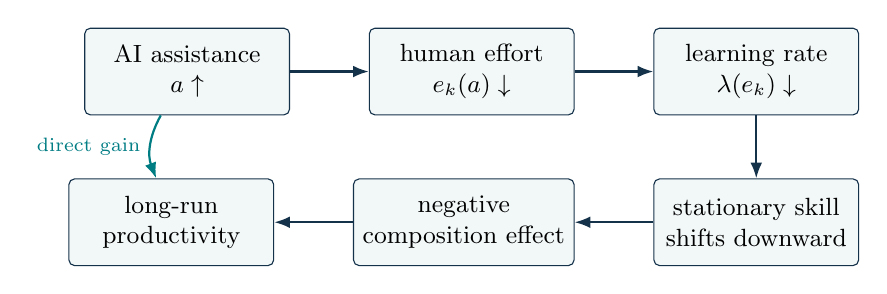
\begin{tikzpicture}[
  node distance=8mm and 10mm,
  box/.style={draw=navy,rounded corners=2pt,fill=pale,minimum width=26mm,
    minimum height=11mm,align=center,font=\small},
  arr/.style={-{Latex[length=2mm]},thick,navy}]
\node[box] (ai) {AI assistance\\$a\uparrow$};
\node[box,right=of ai] (eff) {human effort\\$e_k(a)\downarrow$};
\node[box,right=of eff] (learn) {learning rate\\$\lambda(e_k)\downarrow$};
\node[box,below=of learn] (skill) {stationary skill\\shifts downward};
\node[box,left=of skill] (comp) {negative\\composition effect};
\node[box,left=of comp] (prod) {long-run\\productivity};
\draw[arr] (ai)--(eff);
\draw[arr] (eff)--(learn);
\draw[arr] (learn)--(skill);
\draw[arr] (skill)--(comp);
\draw[arr] (comp)--(prod);
\draw[-{Latex[length=2mm]},thick,teal] (ai) to[bend right=25]
  node[left,font=\scriptsize,teal]{direct gain} (prod);
\end{tikzpicture}
\vspace{5mm}
\bottomline{The theorem compares the positive direct path with the negative learning path.}
\end{frame}

% ============================================================
% RATES AND STATIONARITY
% ============================================================

\begin{frame}[plain]
  \begin{tikzpicture}[remember picture,overlay]
    \fill[navy] (current page.south west) rectangle (current page.north east);
    \fill[teal] (current page.south west) rectangle ([xshift=18mm]current page.north west);
  \end{tikzpicture}
  \vspace{23mm}
  {\color{white}\Huge\bfseries From effort to long-run skill\par}
  \vspace{8mm}
  {\color{white!82}\Large Rates tell us how quickly the agent moves; stationary probabilities tell us where the agent spends time.\par}
\end{frame}

\begin{frame}{A transition rate is a speed, not a probability}
If the agent is currently at $s_i$, then over a very short interval $h$,
\[
\Pr\{S(t+h)=s_j\mid S(t)=s_i\}
=r_{ij}h+o(h).
\]
\econmeaning{$r_{ij}$ is the arrival speed of the move from $i$ to $j$. The probability over a short interval is approximately rate $\times$ interval length.}
\begin{exampleblock}{Why can a rate exceed one?}
A rate is measured per unit of time. A rate of $3$ per year does not mean a probability of $3$; over one week, the probability is approximately $3/52$.
\end{exampleblock}
\end{frame}

\begin{frame}{The model has an upward clock and a downward clock}
At skill state $s_k$,
\[
\boxed{s_k\to s_{k+1}\text{ at rate }\lambda(e_k(a)),
\qquad
s_k\to s_{k-1}\text{ at rate }\mu.}
\]
\econmeaning{Effort controls the speed of skill improvement. Skill depreciation arrives at the constant speed $\mu>0$.}
\bottomline{AI affects upward movement through effort, but it does not change the downward clock directly.}
\end{frame}

\begin{frame}{Competing clocks turn rates into intuitive probabilities}
At an interior state, write $\lambda_k=\lambda(e_k(a))$. Then
\[
\Pr(\text{next move is up})=\frac{\lambda_k}{\lambda_k+\mu},
\qquad
\Pr(\text{next move is down})=\frac{\mu}{\lambda_k+\mu}.
\]
The expected waiting time until either move is
\[
\frac{1}{\lambda_k+\mu}.
\]
\econmeaning{A larger upward rate makes the next change more likely to be an improvement and makes that change arrive sooner.}
\end{frame}

\begin{frame}{Skill moves along a birth--death ladder}
\centering
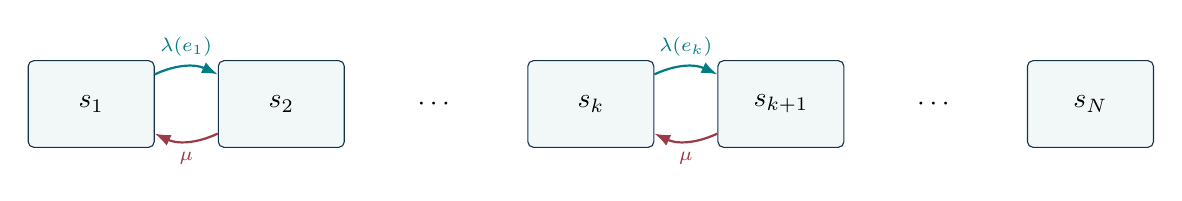
\begin{tikzpicture}[
  node distance=8mm,
  state/.style={draw=navy,rounded corners=2pt,fill=pale,minimum width=16mm,
    minimum height=11mm,align=center},
  up/.style={-{Latex[length=2mm]},bend left=25,thick,teal},
  down/.style={-{Latex[length=2mm]},bend left=25,thick,rose}]
\node[state] (s1) {$s_1$};
\node[state,right=of s1] (s2) {$s_2$};
\node[right=of s2] (dots) {$\cdots$};
\node[state,right=of dots] (sk) {$s_k$};
\node[state,right=of sk] (skp) {$s_{k+1}$};
\node[right=of skp] (dots2) {$\cdots$};
\node[state,right=of dots2] (sn) {$s_N$};
\draw[up] (s1) to node[above,font=\scriptsize] {$\lambda(e_1)$} (s2);
\draw[down] (s2) to node[below,font=\scriptsize] {$\mu$} (s1);
\draw[up] (sk) to node[above,font=\scriptsize] {$\lambda(e_k)$} (skp);
\draw[down] (skp) to node[below,font=\scriptsize] {$\mu$} (sk);
\end{tikzpicture}
\vspace{7mm}
\econmeaning{Only neighboring skill moves are possible. Reaching a distant high-skill state requires a sequence of successful upward transitions.}
\end{frame}

\begin{frame}{Stationary probability is a long-run time share}
Fix the AI level $a$. Define
\[
\boxed{\pi_k(a)=\text{long-run fraction of time spent at skill }s_k.}
\]
The probabilities satisfy
\[
\pi_k(a)\ge0,
\qquad
\sum_{k=1}^{N}\pi_k(a)=1.
\]
\econmeaning{Stationarity does not mean the agent stops moving. It means that probability inflow and outflow balance, so the distribution no longer changes over time.}
\end{frame}

\begin{frame}{Detailed balance is an accounting identity for flows}
Across the edge between $s_k$ and $s_{k+1}$,
\[
\boxed{\pi_k(a)\lambda(e_k(a))
=\pi_{k+1}(a)\mu.}
\]
\begin{columns}[T,onlytextwidth]
\column{.48\textwidth}
\key{Left-hand side}

mass at $s_k$ $\times$ upward speed

$=$ upward flow per unit time.
\column{.48\textwidth}
\key{Right-hand side}

mass at $s_{k+1}$ $\times$ downward speed

$=$ downward flow per unit time.
\end{columns}
\bottomline{In the long run, traffic across each edge must be equal in both directions.}
\end{frame}

\begin{frame}{The adjacent probability ratio summarizes one edge}
Divide detailed balance by $\pi_k(a)\mu>0$:
\[
\boxed{\frac{\pi_{k+1}(a)}{\pi_k(a)}
=\frac{\lambda(e_k(a))}{\mu}.}
\]
\econmeaning{The relative mass on the higher state rises when learning is faster and falls when depreciation is faster.}
\begin{exampleblock}{Reading the ratio}
If $\lambda(e_k)/\mu=2$, state $s_{k+1}$ receives twice as much stationary mass as state $s_k$. If the ratio is $1/2$, it receives half as much.
\end{exampleblock}
\end{frame}

\begin{frame}{The product formula accumulates the odds of every climb}
Repeatedly applying the adjacent ratio gives
\[
\boxed{\pi_k(a)=\pi_1(a)
\prod_{i=1}^{k-1}\frac{\lambda(e_i(a))}{\mu}.}
\]
\econmeaning{To reach state $s_k$ from the bottom, the process must cross every earlier edge. Each factor records how favorable one of those climbs is relative to decay.}
\bottomline{A reduction in an early learning rate affects the stationary weight of every state above that edge.}
\end{frame}

\begin{frame}{Normalization turns positive weights into probabilities}
The product formula determines probabilities only up to the common factor $\pi_1(a)$. The condition $\sum_k\pi_k=1$ gives
\[
\boxed{\pi_1(a)=
\left[
1+\sum_{k=2}^{N}\prod_{i=1}^{k-1}
\frac{\lambda(e_i(a))}{\mu}
\right]^{-1}.}
\]
\econmeaning{The expression in brackets is the total unnormalized mass. Its reciprocal rescales all weights so that they sum to one. The exponent $-1$ simply means ``take the reciprocal.''}
\end{frame}

\begin{frame}{A two-state example makes the stationary logic concrete}
Suppose
\[
\lambda_1=0.30,
\qquad
\mu=0.10.
\]
Then detailed balance implies
\[
0.30\pi_1=0.10\pi_2
\quad\Longrightarrow\quad
\pi_2=3\pi_1.
\]
Together with $\pi_1+\pi_2=1$,
\[
\boxed{(\pi_1,\pi_2)=(0.25,0.75).}
\]
\econmeaning{An upward clock three times faster than the downward clock places three times as much long-run mass on the high-skill state.}
\end{frame}

\begin{frame}{Long-run outcomes are stationary weighted averages}
At state $s_k$, effort is $e_k(a)$ and productivity is $p_k^\star(a)$. Therefore
\[
\boxed{\calE(a)=\sum_{k=1}^{N}\pi_k(a)e_k(a),
\qquad
\calP(a)=\sum_{k=1}^{N}\pi_k(a)p_k^\star(a).}
\]
\econmeaning{A state contributes more to a long-run average when the process spends more time there. Both the state outcomes and the time shares may respond to AI.}
\end{frame}

% ============================================================
% SKILL DEGRADATION
% ============================================================

\begin{frame}[plain]
  \begin{tikzpicture}[remember picture,overlay]
    \fill[navy] (current page.south west) rectangle (current page.north east);
    \fill[rose] (current page.south west) rectangle ([xshift=18mm]current page.north west);
  \end{tikzpicture}
  \vspace{23mm}
  {\color{white}\Huge\bfseries Why more AI lowers long-run skill\par}
  \vspace{8mm}
  {\color{white!82}\Large The proof is an ordered comparison of adjacent stationary odds.\par}
\end{frame}

\begin{frame}{More AI weakly lowers effort at every skill state}
For $a_\ell<a_h$,
\[
e_i(a_\ell)=\pos{x^\star-s_i-a_\ell}
\ge
\pos{x^\star-s_i-a_h}=e_i(a_h).
\]
Since $\lambda$ is increasing,
\[
\boxed{\lambda(e_i(a_\ell))\ge\lambda(e_i(a_h))
\quad\text{for every }i.}
\]
\econmeaning{Lower AI preserves at least as much human effort at every skill level, so every upward learning clock is at least as fast.}
\end{frame}

\begin{frame}{Every adjacent stationary odds ratio moves against high skill}
Let
\[
r_i(a):=\frac{\pi_{i+1}(a)}{\pi_i(a)}
=\frac{\lambda(e_i(a))}{\mu}.
\]
Then $a_\ell<a_h$ implies
\[
\boxed{r_i(a_\ell)\ge r_i(a_h)
\quad\text{for every edge }i.}
\]
\econmeaning{Moving from low AI to high AI makes every step up the skill ladder less favorable relative to the step down.}
\end{frame}

\begin{frame}{First-order stochastic dominance formalizes ``more high skill''}
The low-AI distribution dominates the high-AI distribution when
\[
\boxed{
\sum_{i=1}^{k}\pi_i(a_\ell)
\le
\sum_{i=1}^{k}\pi_i(a_h)
\quad\text{for every }k.}
\]
\econmeaning{For every cutoff $s_k$, low AI gives a smaller probability of being at or below that cutoff. Equivalently, it places more mass on high skill.}
\begin{alertblock}{Read the inequality in the correct direction}
The states are ordered from low to high. A smaller lower-tail probability means a better skill distribution.
\end{alertblock}
\end{frame}

\begin{frame}{A three-state example shows the downward shift}
Suppose the adjacent ratios are
\[
(r_1^\ell,r_2^\ell)=(2,1.5),
\qquad
(r_1^h,r_2^h)=(1,0.75).
\]
The unnormalized weights are therefore
\[
w^\ell=(1,2,3),
\qquad
w^h=(1,1,0.75).
\]
After normalization,
\[
\pi^\ell=\left(\frac16,\frac13,\frac12\right),
\qquad
\pi^h=\left(\frac4{11},\frac4{11},\frac3{11}\right).
\]
\econmeaning{High AI roughly doubles the probability of the lowest state and nearly halves the probability of the highest state.}
\end{frame}

\begin{frame}{Deskilling is certain; lower productivity is not}
The skill result is unambiguous:
\[
a\uparrow
\quad\Longrightarrow\quad
\text{stationary skill distribution shifts downward}.
\]
But productivity contains two forces:
\[
\underbrace{p_k^\star(a)\uparrow}_{\text{direct gain}}
\qquad\text{and}\qquad
\underbrace{\pi(a)\text{ shifts down}}_{\text{composition loss}}.
\]
\bottomline{Skill degradation is the mechanism that makes a paradox possible, not a sufficient condition for the paradox by itself.}
\end{frame}

% ============================================================
% ACTIVITY REGIMES AND SENSITIVITY GAP
% ============================================================

\begin{frame}[plain]
  \begin{tikzpicture}[remember picture,overlay]
    \fill[navy] (current page.south west) rectangle (current page.north east);
    \fill[gold] (current page.south west) rectangle ([xshift=18mm]current page.north west);
  \end{tikzpicture}
  \vspace{23mm}
  {\color{white}\Huge\bfseries When does deskilling dominate?\par}
  \vspace{8mm}
  {\color{white!82}\Large Activity regimes isolate a smooth comparison between the direct and learning channels.\par}
\end{frame}

\begin{frame}{Active effort states always form a lower block}
Effort is positive exactly when
\[
e_k(a)>0
\quad\Longleftrightarrow\quad
s_k+a<x^\star.
\]
Because $s_1\le\cdots\le s_N$, if state $s_k$ is active, then every lower state is active too.
\[
\boxed{\text{Active states}=\{1,\ldots,m\}
\quad\text{for some }m.}
\]
\econmeaning{High-skill agents stop exerting effort first because their baseline input reaches the target $x^\star$ sooner.}
\end{frame}

\begin{frame}{An activity interval keeps the same states active}
Define
\[
\boxed{I_m=
\bigl((x^\star-s_{m+1})^+,(x^\star-s_m)^+\bigr].}
\]
For $a$ inside $I_m$,
\[
e_k(a)>0\ (k\le m),
\qquad
e_k(a)=0\ (k\ge m+1).
\]
\econmeaning{Inside one interval, no state switches formula. This lets us compare the two economic forces without being distracted by kinks at effort zero.}
\end{frame}

\begin{frame}{Active and inactive states react differently to AI}
Inside $I_m$,
\[
p_k^\star(a)=
\begin{cases}
p(x^\star), & k\le m,\\
p(s_k+a), & k\ge m+1.
\end{cases}
\]
\begin{columns}[T,onlytextwidth]
\column{.48\textwidth}
\key{Active states}

AI replaces effort. Output stays fixed, but learning slows.
\column{.48\textwidth}
\key{Inactive states}

Effort is already zero. AI directly raises output.
\end{columns}
\bottomline{The paradox is created by the coexistence of replacement states and expansion states.}
\end{frame}

\begin{frame}{The aggregate derivative has a gain and a composition term}
Differentiate the stationary average:
\[
\boxed{
\calP'(a)=
\underbrace{\sum_{k=1}^{N}\pi_k(a)\frac{d p_k^\star(a)}{da}}
_{\text{within-state direct gain }\ge0}
+
\underbrace{\sum_{k=1}^{N}\pi_k'(a)p_k^\star(a)}
_{\text{composition effect}}.}
\]
Because $\sum_k\pi_k'(a)=0$, the second term only reallocates mass between states.
\econmeaning{The direct effect asks what changes within each skill group. The composition effect asks how the population moves across groups.}
\end{frame}

\begin{frame}{The sensitivity gap compares proportional responses}
At the right endpoint of regime $I_m$, define
\[
\boxed{
\Delta_m=
\underbrace{\sum_{j=1}^{m}
\frac{\lambda'(s_m-s_j)}{\lambda(s_m-s_j)}}
_{\text{learning-weight sensitivity}}
-
\underbrace{
\frac{p'(x^\star+s_{m+1}-s_m)}
{p(x^\star+s_{m+1}-s_m)-p(x^\star)}}
_{\text{productivity-premium sensitivity}}.}
\]
\econmeaning{$\Delta_m$ is not a level comparison. It compares how rapidly the learning channel and the direct productivity channel respond locally to one more unit of AI.}
\end{frame}

\begin{frame}{The first term asks how fragile learning weights are}
For a positive function $f$,
\[
\frac{f'(x)}{f(x)}=\frac{d}{dx}\log f(x).
\]
Therefore,
\[
\sum_{j=1}^{m}\frac{\lambda'(s_m-s_j)}{\lambda(s_m-s_j)}
\]
is the combined proportional sensitivity of the active learning rates.
\econmeaning{If this term is large, a small reduction in effort causes a large percentage reduction in the stationary weights supporting higher skill.}
\end{frame}

\begin{frame}{The second term asks how responsive the AI premium is}
Let
\[
R_m=p(x^\star+s_{m+1}-s_m)-p(x^\star)>0.
\]
Then
\[
\frac{p'(x^\star+s_{m+1}-s_m)}{R_m}
\]
is the marginal direct gain relative to the existing productivity premium.
\econmeaning{If this term is large, additional AI expands output rapidly in the first inactive state. The direct productivity channel is then difficult for deskilling to overturn.}
\end{frame}

\begin{frame}{A positive gap means learning is locally more sensitive}
\[
\boxed{\Delta_m>0
\quad\Longleftrightarrow\quad
\text{learning sensitivity}>
\text{productivity sensitivity}.}
\]
\begin{columns}[T,onlytextwidth]
\column{.48\textwidth}
\begin{block}{$\Delta_m>0$}
The negative learning channel can dominate when skill decay is sufficiently fast.
\end{block}
\column{.48\textwidth}
\begin{exampleblock}{$\Delta_m<0$}
The direct productivity channel is locally more sensitive, so productivity remains increasing in the theorem's regime.
\end{exampleblock}
\end{columns}
\bottomline{The sign identifies which channel is more responsive; $\mu$ determines how strongly that responsiveness enters stationary outcomes.}
\end{frame}

\begin{frame}{The decay rate controls the economic importance of learning}
The key relative rate is
\[
\frac{\lambda(e_k(a))}{\mu}.
\]
\begin{columns}[T,onlytextwidth]
\column{.48\textwidth}
\key{Small $\mu$}

Skill is persistent. The process spends most time near high skill, so modest learning changes have limited aggregate impact.
\column{.48\textwidth}
\warning{Large $\mu$}

Skill depreciates rapidly. Maintaining high skill requires repeated learning, so reduced effort becomes consequential.
\end{columns}
\bottomline{$\Delta_m>0$ creates the vulnerable margin; sufficiently large $\mu$ makes that margin visible in long-run productivity.}
\end{frame}

\begin{frame}{Within one regime, productivity can turn only once}
The paper proves that on every nonempty $I_m$,
\[
\boxed{\calP(a)\text{ is either increasing everywhere,
or increasing and then decreasing}.}
\]
\econmeaning{As AI rises within a regime, the marginal direct gain becomes weaker while the composition loss becomes relatively stronger. Once the derivative turns negative, it cannot turn positive again before the next activity boundary.}
\begin{alertblock}{Why regime boundaries matter}
At a boundary, one state stops exerting effort and changes from the replacement formula to the expansion formula. The derivative may therefore reset.
\end{alertblock}
\end{frame}

\begin{frame}{The theorem converts intuition into a shape result}
For sufficiently large $\mu$ and a nonempty activity interval $I_m$:
\begin{block}{Paper's Theorem 1}
\begin{enumerate}
  \item If $1\le m\le N-1$ and $\Delta_m>0$, then $\calP$ increases and then decreases on $I_m$.
  \item If $m\in\{0,N\}$ or $\Delta_m<0$, then $\calP$ is weakly increasing on $I_m$.
\end{enumerate}
\end{block}
\bottomline{The paradox requires an intermediate regime, a positive sensitivity gap, and sufficiently rapid skill decay.}
\end{frame}

\begin{frame}{The two boundary regimes cannot create the paradox}
\begin{columns}[T,onlytextwidth]
\column{.48\textwidth}
\begin{block}{$I_N$: all states active}
Every state fills the gap to $x^\star$:
\[
p_k^\star(a)=p(x^\star).
\]
Hence $\calP(a)=p(x^\star)$ is flat.
\end{block}
\column{.48\textwidth}
\begin{exampleblock}{$I_0$: all states inactive}
Every effort is zero, so learning rates are fixed at $\lambda(0)$:
\[
\calP'(a)=\sum_k\pi_k p'(s_k+a)\ge0.
\]
\end{exampleblock}
\end{columns}
\econmeaning{A decline needs some states to lose learning effort while other states receive a direct AI productivity gain.}
\end{frame}

% ============================================================
% TWO STATES AND REVERSAL
% ============================================================

\begin{frame}[plain]
  \begin{tikzpicture}[remember picture,overlay]
    \fill[navy] (current page.south west) rectangle (current page.north east);
    \fill[teal] (current page.south west) rectangle ([xshift=18mm]current page.north west);
  \end{tikzpicture}
  \vspace{23mm}
  {\color{white}\Huge\bfseries Two states reveal the entire paradox\par}
  \vspace{8mm}
  {\color{white!82}\Large One learning rate, one decay rate, and one changing composition weight are enough.\par}
\end{frame}

\begin{frame}{In the intermediate regime, one state learns and one expands}
For $N=2$ and $a\in I_1=(x^\star-s_2,x^\star-s_1]$,
\[
e_1(a)=x^\star-s_1-a,
\qquad
e_2(a)=0.
\]
Define $L(a)=\lambda(e_1(a))$. Then
\[
\boxed{\pi_1(a)=\frac{\mu}{\mu+L(a)},
\qquad
\pi_2(a)=\frac{L(a)}{\mu+L(a)}.}
\]
\econmeaning{Higher AI lowers $L(a)$, so stationary mass moves from the productive high-skill state $s_2$ toward the low-skill state $s_1$.}
\end{frame}

\begin{frame}{Two-state productivity is a transparent weighted average}
State 1 remains at the target output $P_0=p(x^\star)$, while state 2 produces $P_2(a)=p(s_2+a)$. Thus
\[
\boxed{
\calP(a)=
\frac{\mu P_0+L(a)P_2(a)}{\mu+L(a)}.}
\]
\econmeaning{AI raises $P_2(a)$ directly, but it simultaneously lowers the weight $L(a)/(\mu+L(a))$ placed on that high-productivity state.}
\bottomline{The whole paradox is visible in one quotient: the payoff rises while its weight falls.}
\end{frame}

\begin{frame}{The exact two-state threshold separates the two forces}
Let
\[
d=s_2-s_1,
\quad
R=p(x^\star+d)-p(x^\star),
\quad
p'_R=p'(x^\star+d).
\]
When $\Delta_1>0$, define
\[
\boxed{
\bar\mu_2=
\frac{\lambda(0)^2p'_R}
{\lambda'(0)R-\lambda(0)p'_R}.}
\]
\econmeaning{The denominator is positive exactly when learning is more sensitive than the direct productivity premium. The numerator scales the remaining direct gain.}
\end{frame}

\begin{frame}{Two conditions produce the N-shaped response}
For two states:
\[
\boxed{\Delta_1>0
\quad\text{and}\quad
\mu>\bar\mu_2}
\]
imply the global sequence
\[
\text{flat}
\quad\longrightarrow\quad
\text{rising}
\quad\longrightarrow\quad
\text{falling}
\quad\longrightarrow\quad
\text{rising}.
\]
\econmeaning{At low AI, effort absorbs assistance and output is flat. In the intermediate regime, direct gains initially win and deskilling later wins. At high AI, effort is already zero, so only direct gains remain.}
\end{frame}

\begin{frame}{A numerical calibration gives a concrete threshold}
Use
\[
\lambda(e)=1+e,
\qquad
p(x)=\log(1+x),
\qquad
x^\star=3,
\qquad
(s_1,s_2)=(0,2).
\]
Then
\[
R=\log 6-\log 4\approx0.4055,
\qquad
p'_R=\frac16,
\]
and
\[
\boxed{\bar\mu_2
=\frac{1/6}{0.4055-1/6}
\approx0.698.}
\]
\econmeaning{With $\mu=1$, a declining subregion exists. With $\mu=0.5$, memory is persistent enough that productivity remains increasing.}
\end{frame}

\begin{frame}{The productivity shortfall can be arbitrarily severe}
The paper proves that for every $\varepsilon>0$, one can choose valid primitives such that
\[
\boxed{
\inf_{a_\ell<a_h}
\frac{\calP(a_h)}{\calP(a_\ell)}
\le\varepsilon.}
\]
\econmeaning{This is an existence result. It says the model does not impose a universal lower bound on the damage from deskilling; it does not predict a severe decline for every empirical setting.}
\begin{exampleblock}{Construction intuition}
Make zero-effort learning almost impossible, but let a small amount of effort be enough to sustain high-skill stationary mass.
\end{exampleblock}
\end{frame}

\begin{frame}{Simpson's paradox is the right aggregation analogy}
Differentiate the aggregate:
\[
\boxed{
\calP'(a)=
\underbrace{\sum_k\pi_k(a)p_k^{\star\prime}(a)}_{\text{within-state effect }\ge0}
+
\underbrace{\sum_k\pi_k'(a)p_k^\star(a)}_{\text{composition effect}}.}
\]
\econmeaning{Every skill group can improve while the aggregate falls, because AI changes the shares of the groups. The reversal comes from endogenous weights.}
\bottomline{The model's paradox is Simpson-type: the direction within groups differs from the direction after aggregation.}
\end{frame}

\begin{frame}{A numerical Simpson reversal needs almost no algebra}
Under low AI, suppose
\[
\pi^\ell=(0.25,0.75),
\qquad
p^\ell=(10,16),
\qquad
\calP_\ell=14.5.
\]
Under high AI, both state productivities rise by one, but the weights reverse:
\[
\pi^h=(0.75,0.25),
\qquad
p^h=(11,17),
\qquad
\boxed{\calP_h=12.5<14.5.}
\]
\econmeaning{Each group gains one unit, yet the population spends much more time in the low-productivity group. The composition loss is three units, which dominates the direct gain of one.}
\end{frame}

\begin{frame}{Exogenous transition rates remove the paradox}
If upward rates are fixed numbers $\lambda_k$ rather than functions of effort, then
\[
\pi_k'(a)=0.
\]
Therefore,
\[
\boxed{
\calP'(a)=\sum_{k=1}^{N}\pi_k
\frac{d p_k^\star(a)}{da}\ge0.}
\]
\econmeaning{Heterogeneous skill alone is not enough. The paradox requires AI to change effort, effort to change learning, and learning to change the long-run skill distribution.}
\end{frame}

\begin{frame}{The complete causal chain has two competing paths}
\centering
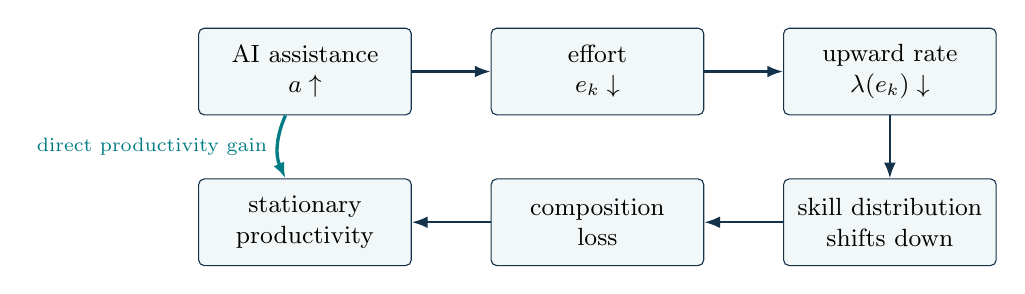
\begin{tikzpicture}[
  node distance=8mm and 10mm,
  box/.style={draw=navy,rounded corners=2pt,fill=pale,minimum width=27mm,
    minimum height=11mm,align=center,font=\small},
  arr/.style={-{Latex[length=2mm]},thick,navy}]
\node[box] (ai) {AI assistance\\$a\uparrow$};
\node[box,right=of ai] (eff) {effort\\$e_k\downarrow$};
\node[box,right=of eff] (rate) {upward rate\\$\lambda(e_k)\downarrow$};
\node[box,below=of rate] (dist) {skill distribution\\shifts down};
\node[box,left=of dist] (loss) {composition\\loss};
\node[box,left=of loss] (P) {stationary\\productivity};
\draw[arr] (ai)--(eff);
\draw[arr] (eff)--(rate);
\draw[arr] (rate)--(dist);
\draw[arr] (dist)--(loss);
\draw[arr] (loss)--(P);
\draw[-{Latex[length=2mm]},very thick,teal] (ai) to[bend right=24]
 node[left,font=\scriptsize,teal]{direct productivity gain} (P);
\end{tikzpicture}
\vspace{5mm}
\begin{block}{How to read the theorem}
$\Delta_m$ compares the local sensitivities of the two paths. The decay rate $\mu$ determines how strongly the learning path affects long-run weights.
\end{block}
\end{frame}

\begin{frame}{Six conclusions to carry out of Part II}
\begin{enumerate}
  \item AI and effort are perfect substitutes in the static problem.
  \item Effort is an input into skill development through $\lambda(e)$.
  \item More AI lowers every upward stationary odds ratio and shifts skill downward.
  \item Aggregate productivity combines a positive direct effect and a potentially negative composition effect.
  \item A positive sensitivity gap and sufficiently rapid decay create a declining region.
  \item The paradox disappears when transition rates are exogenous.
\end{enumerate}
\vspace{3mm}
\bottomline{The central message is not ``AI lowers productivity.'' It is that static gains do not determine long-run outcomes when the weights are endogenous.}
\end{frame}

\begin{frame}{Questions that test economic understanding}
\begin{enumerate}
  \item Why is $\lambda(e)$ a rate rather than a probability?
  \item Why does $\pi_{k+1}/\pi_k=\lambda(e_k)/\mu$ summarize one skill edge?
  \item Why does lower AI first-order stochastically dominate higher AI?
  \item Why is deskilling not sufficient by itself for a productivity decline?
  \item What distinct roles do $\Delta_m$ and $\mu$ play?
  \item Why can the derivative become positive again after an activity boundary?
  \item What assumption does the exogenous-transition benchmark remove?
\end{enumerate}
\vspace{3mm}
\centering
\large A strong answer should describe the economic mechanism before manipulating the equation.
\end{frame}

\begin{frame}{References and scope}
\small
\textbf{Primary paper}

Ali Aouad, Thodoris Lykouris, and Huiying Zhong.
\emph{Human--AI Productivity Paradoxes: Modeling the Interplay of Skill, Effort, and AI Assistance}.
arXiv:2605.11350v1, 2026.

\vspace{5mm}
\textbf{Probability background}

Geoffrey Grimmett and David Stirzaker.
\emph{Probability and Random Processes}, 3rd ed. Oxford University Press, 2001.

\vspace{5mm}
\begin{block}{Deck scope}
This lecture covers endogenous skill development and the first productivity paradox. It emphasizes interpretation rather than reproducing every algebraic step in the longer tutorial.
\end{block}
\vfill
\centering
\href{mailto:aquisper@caltech.edu}{aquisper@caltech.edu}
\end{frame}

\end{document}
